\documentclass{article}

\title{Estatística Numérica Computacional\\Trabalho nº4}
\author{Marta Paz nº49861\\
		Rafael Almeida nº49788\\
		Rafael Gameiro nº50677\\
		Ricardo Pinto nº49811\\
}
\date{December, 2018}

\usepackage{amsmath}
\usepackage{graphicx}
\usepackage{enumerate}
\usepackage{subcaption}
\usepackage{float}

\begin{document}
	\maketitle
	\pagenumbering{gobble}
	\newpage
	\pagenumbering{arabic}
	
	
	\section*{Estimação do parâmetro gama num modelo de crescimento não linear}
		\paragraph{}
			Suponha que estamos interessados em considerar um modelo de crescimento não linear de uma espécie de animais em que o crescimento de cada animal \textit{Y} se relaciona com a sua idade \textit{x}. Assim, para o animal \textit{i}, o modelo postula que: \\

			\textit{$Y_i$} $\sim Normal \left(\alpha - \beta \gamma^{x_i} , \sigma^2 \right), \alpha, \beta > 0; \indent 0 < \gamma < 1$.\\
			
			Considere que $\alpha = 2.7$, que $\beta = 0.9$ e que $\sigma^2 = 0.01$. \\
			\indent Assuma uma distribuição \textit{a priori} não informativa Uniforme(0,1) para $\gamma$. \\
			\indent Considere ainda os dados observados: \\

			\textit{x} = (1.0, 1.5, 1.5, 1.5, 2.5, 4.0, 5.0, 5.0, 7.0, 8.0, 8.5, 9.0, 9.5, 9.5, 10.0, 12.0, 12.0, 13.0, 13.0, 14.5, 15.5, 15.5, 16.5, 17.0, 22.5, 29.0, 31.5) \\

			\textit{Y} = (1.80, 1.85, 1.87, 1.77, 2.02, 2.27, 2.15, 2.26, 2.47, 2.19, 2.26, 2.40, 2.39, 2.41, 2.50, 2.32, 2.32, 2.43, 2.47, 2.56, 2.65, 2.47, 2.64, 2.56, 2.70, 2.72, 2.57) \\
			

		\subsection*{Alínea 1}
			\paragraph{}
				Obtenha a densidade \textit{a posteriori} de $\gamma$, a menos de uma constante multiplicativa. 

			\subsection*{Resolução}
				\paragraph{}
					A probabilidade \textit{a posteriori} consiste no cálculo de uma probabilidade condicionada aplicada a um conjunto de dados anteriormente tratados. A distribuição \textit{a posteriori} descreve, assim, todo o conhecimento que se tem no momento à cerca de uma variável, com base na informação obtida \textit{a priori} segundo uma função de verosimilhança.\\
					Por outras palavras, a distribuição de probabilidade \textit{a posteriori} de uma variável aleatória \textit{x}, sabendo o valor de uma outra variável $\theta$, que resulta na função densidade de probabilidade \textit{a posteriori} de $\Theta$, pode ser calculada pelo Teorema de Bayes:
					\begin{align*}
						h(\theta\mid\textit{x}) = \frac { f(\textit{x}\mid\theta)  h(\theta) } { \int_{\theta}^{}  f(\textit{x}\mid\theta)  h(\theta) } \\
					\end{align*}	

					Sejam, portanto: \\
					\indent $h(\theta\mid\textit{x})$ - densidade \textit{a posteriori} de $\theta$ \\
					\indent $h(\theta)$ - densidade \textit{a priori} de $\theta$ \\
					\indent $f(\textit{x}\mid\theta)$ - função de verosimilhança de \textit{x} sabendo $\theta$ \\

					Seja ainda:
					
					\begin{align*}
						f(\textit{x}) =  \int_{\theta}^{}  f(\textit{x}\mid\theta)  h(\theta) dx
					\end{align*}

					Uma vez que f(\textit{x}) não depende de $\theta$, podemos assumir que: \\
					$h(\theta\mid\textit{x})$ = $\frac { f(\textit{x}\mid\theta)  h(\theta) } { \int_{\theta}^{}  f(\textit{x}\mid\theta)  h(\theta) dx }$ é, na verdade, proporcional a $f(\textit{x}\mid\theta)  h(\theta)$ \\

					Nesta alínea é pedido para calcularmos a densidade \textit{a posteriori} de $\gamma$. \\
					Substituindo, na fórmula da densidade \textit{a posteriori}, pelas variáveis correspondentes ao enunciado, temos: 

					\begin{align*}
						h(\gamma\mid\textit{y}) = \frac { f(\textit{y}\mid\gamma)  h(\gamma) } { \int_{\gamma}^{}  f(\textit{y}\mid\gamma)  h(\gamma) } 
					\end{align*}

					Sabe-se que $h(\gamma)$ assume uma distribuição \textit{Uniforme(0,1)} e que $f(\textit{y}\mid\gamma)$ assume uma distribuição \textit{Normal}. Assim sendo, temos as respetivas funções densidade de probabilidade (f.d.p.): \\

					- f.d.p. da Distribuição Uniforme:\\
					\textit{Uniforme(a,b)} $\Rightarrow$ \textit{Uniforme(0,1)}: \\
					\begin{align*}
						f(\textit{y}) = \frac{1}{b-a}\Rightarrow \frac{1}{1-0} = 1 
					\end{align*} 

					- f.d.p. da Distribuição Normal:\\
					Normal($\mu$,$\sigma^2$) $\Rightarrow$ Normal($\alpha$ - $\beta\gamma^x$, $\sigma^2$) $\Rightarrow$ Normal(2,7 - 0,9$\gamma^x$, 0,01):\\
					
					\begin{equation*}
						\frac{1}{\sqrt{2\pi}\sigma}e^{-\frac{(y-\mu)^2}{2\sigma^2}} \Leftrightarrow \frac{1}{\sqrt{2\pi}\sigma}e^{-\frac{(y-2.7+0.9\gamma^{x_{i}})^2}{2*0.01}}
					\end{equation*}
			\paragraph{}
					
	Substituindo estas funções densidade na função de densidade \textit{a posteriori}, obtemos:
					\begin{align*}
						h(\gamma|y) = \frac{\frac{1}{\sqrt{2\pi}\sigma}e^{-\frac{(y-2.7+0.9\gamma^{x})^2}{2*0.01}}*1}{\int_{}^{}{\frac{1}{\sqrt{2\pi}\sigma}e^{-\frac{(y-2.7+0.9\gamma^x)^2}{2*0.01}}} *1 d\gamma} 
								= \frac{\frac{1}{\sqrt{2\pi}\sigma}e^{-\frac{(y-2.7+0.9\gamma^{x})^2}{2*0.01}}}{\frac{1}{\sqrt{2\pi}\sigma}\int_{}^{}{e^{-\frac{(y-2.7+0.9\gamma^x)^2}{2*0.01}}}  d\gamma} 
								= \frac{e^{-\frac{(y-2.7+0.9\gamma^{x})^2}{2*0.01}}}{\int_{}^{}{e^{-\frac{(y-2.7+0.9\gamma^x)^2}{2*0.01}}}  d\gamma}
					\end{align*}

	Esta fórmula é proporcional a:
					\begin{align*}
						h(\gamma | y ) \propto e^{-\frac{(y-2.7+0.9\gamma^x)^2}{2*0.01}}
					\end{align*}
					
	Uma vez que as variáves dependem de vários valores, temos que:
					\begin{align*}
						h(\gamma | y) \propto \prod_{i=1}^{n=27}e^{-\frac{(y_{i}-2.7+0.9\gamma^{x_{i}})^2}{2*0.01}} = e^{\sum_{i=1}^{n=27}-\frac{(y_{i}-2.7+0.9\gamma^{x_{i}})^2}{2*0.01}}
					\end{align*}


		\subsection*{Alínea 2}
			\paragraph{}
				Estabeleça um algoritmo do \textit{método de Metropolis-Hastings} para amostrar da distribuição \textit{a posteriori} de $\gamma$. Analise e comente os resultados. Usando valores amostrados através do seu algoritmo, estime a probabilidade \textit{a posteriori} de $\gamma$ tomar valores superiores a 0.9.

			\subsection*{Resolução}
				\paragraph{}
					 O \textit{método de Metropolis-Hastings} pertence aos métodos Markov Chain Monte Carlo (M.C.M.C), e consiste em formar uma cadeia de Markov gerando várias amostras apartir de uma distribuição proposta. Cada valor gerado pode ou não ser aceite com base na densidade da distribuição \textit{a priori}, o que permite que a cadeia, no final, convirja para uma distribuição, a distribuição \textit{a posteriori}. 
		
				Para este exercício, fizemos um algoritmo do \textit{método de Metropolis-Hastings} em R, com o objetivo de amostrar a distribuição \textit{a posteriori} de $\gamma$. Depois de colocar os dados do enunciado no R, na forma de dois vetores, criámos uma função para executar o algoritmo. Essa função recebe como parâmetros os dados x e y, o primeiro valor de gama, o burn.in (valor utilizado para "desprezar" os primeiros valores) e o m (valor que, somado com o burn.in, vai dar origem ao número de valores de gama gerados). Os valores de burn.in, de m e do primeiro gama podem ser fornecidos, mas a função já têm valores pré-definidos. Pelo contrário, os valores de x e y tem de ser obrigatoriamente fornecidos. Depois temos de:
				\begin{enumerate}
					\item Criar a variável gama, que é uma matriz de (burn.in+m) x 1
  					 \item Atribuir o valor recebido como parâmetro do primeiro gama à posição 1 de gama
					 \item Gerar um $\gamma$' com o runif(1)
					 \item Calcular $\alpha$ = min$\left(1,\frac{f(y | \gamma')}{f(y| \gamma )}\right)$ = min$\left(1, \frac{e^{\sum_{i=1}^{n=27}-\frac{(y_{i}-2.7+0.9\gamma'^{x_{i}})^2}{2*0.01}}}{e^{\sum_{i=1}^{n=27}-\frac{(y_{i}-2.7+0.9\gamma^{x_{i}})^2}{2*0.01}}}\right)$ , sendo que $\gamma$' é o $\gamma$' gerado em (3) e $\gamma$ é o elemento da posição gama[i-1]
					\item Gerar um u = runif(1)
					\item Se u $\leq \alpha$, gama[i] = $\gamma$' e a taxa de aceitação é incrementada. Caso contrário gama[i] = gama[i-1]
					\item Fazer os pontos 3 a 6, desde i=2 até burn.in+m 
					\item Quando o ciclo acaba, é retornado os valores de gama compreendidos entre burn.in e m. 
 				\end{enumerate}
				\paragraph{}
				Para estimar a probabilidade \textit{a posteriori} de \textit{$\gamma$} tomar valores superiores a 0.9 temos que:
				
				\paragraph{}
				$\hat{P}$($\gamma$ $>$0.9 $|$ y) = sum(gama.MH\$gama $>$ 0.9 ) / length(gama.MH\$gama) = 0.26789 , em que

				\begin{itemize}
					\item gama.MH\$gama : todos os valores de gama calculados com o algoritmo implementado para o  \textit{método de Metropolis-Hastings}
					\item gama.MH\$gama $>$ 0.9 : os valores de gama maiores que 0.9
					\item sum(gama.MH\$gama $>$ 0.9 ) : o número de valores maiores que 0.9
					\item length(gama.MH\$gama) : o número total de elementos gama calculados
				\end{itemize} 
		
		\subsection*{Análise de Resultados}

		Após correr o algoritmo obtivemos uma taxa de aceitação igual a  0.023. De seguida, calculámos a média e o desvio padrão dos valores obtidos com o algoritmo implementado, resultando em 0.8951985 e 0.007216911, respetivamente. Por último, fizemos o seguinte histograma com base nos valores de gama obtidos com o algoritmo:
				\begin{figure}[!h]
   					 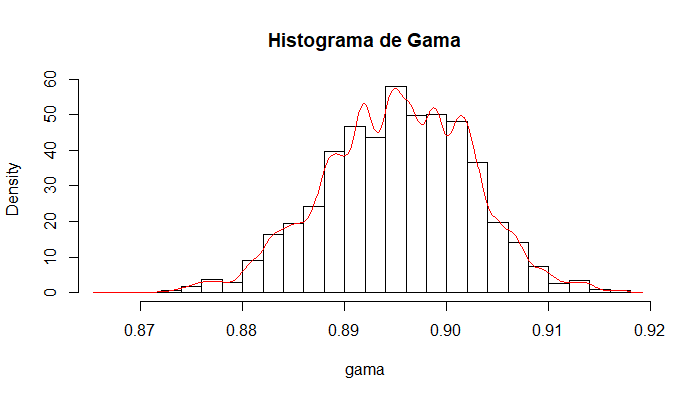
\includegraphics[width=\textwidth]{Histograma}
 				\end{figure}
				

E, analisando o histograma, podemos verificar que a distribuição de $\gamma$ se assemelha com a distribuição Normal($\mu$, $\sigma^2$).

		\subsection*{Alínea 3}
			\paragraph{}
				Um aspeto importante da modelação Bayesiana é a sensibilidade dos resultados à escolha da distribuição \textit{a priori} dos parâmetros desconhecidos. Assim, conduza uma análise de sensibilidade neste sentido considerando outras distribuições \textit{a priori} diferentes para $\gamma$. Escolha essas novas distribuições \textit{a priori} para $\gamma$ na família Beta(a,b), de tal forma que explore as consequências nos resultados de escolher distribuições \textit{a priori} mais e menos variáveis que a inicial.  Relembre que a distribuição Uniforme(0,1) é na verdade uma distribuição Beta(1,1) e consulte o formulário para relembrar quanto valem a média e a variância de variáveis aleatórias com distribuição Beta.

			\subsection*{Resolução}
				\paragraph{}
				Para este exercício é pedido que façamos uma análise de sensibilidade considerando outras distribuições \textit{a priori} para $\gamma$. Essas novas distribuições devem estar na família Beta(a,b), de tal forma que explore as consequências nos resultados de escolher distribuições \textit{a priori} mais e menos variáveis que a inicial.
				\paragraph{}
				Deste modo, baseamos a nossa resposta no algoritmo implementado na alínea anterior. Por isso, começamos por definir a função densidade \textit{a posteriori} para este caso em que a variável $\gamma$ assume uma função de distribuição \textit{a priori} Beta(a,b).
				\paragraph{}
				Assim ficamos com:

				\paragraph{}
				
				\centerline{$h(\gamma|y) = \frac{   \frac{1}{\sqrt{2\pi}\sigma}   \times   e^{-\frac{{(y-2,7+0,9\gamma^{x})}^2}{2\times0,01}}   \times    \frac{1}{Beta(a,b)}   \times   \gamma^{a-1}   \times   (1-\gamma)^{b-1}   }{   \int_{}^{} \frac{1}{\sqrt{2\pi}\sigma}   \times   e^{-\frac{{(y-2,7+0,9\gamma^{x})}^2}{2\times0,01}}   \times    \frac{1}{Beta(a,b)}   \times   \gamma^{a-1}   \times   (1-\gamma)^{b-1} d\gamma   }$ =}

				\paragraph{}
				\centerline{$= \frac{   \frac{1}{\sqrt{2\pi}\sigma}   \times   e^{-\frac{{(y-2,7+0,9\gamma^{x})}^2}{2\times0,01}}   \times    \frac{1}{Beta(a,b)}   \times   \gamma^{a-1}   \times   (1-\gamma)^{b-1}   }{   \frac{1}{\sqrt{2\pi}\sigma}   \times   \int_{}^{} e^{-\frac{{(y-2,7+0,9\gamma^{x})}^2}{2\times0,01}}   \times    \frac{1}{Beta(a,b)}   \times   \gamma^{a-1}   \times   (1-\gamma)^{b-1} d\gamma   }$ =}

				\paragraph{}
				\centerline{$= \frac{   e^{-\frac{{(y-2,7+0,9\gamma^{x})}^2}{2\times0,01}}   \times    \frac{1}{Beta(a,b)}   \times   \gamma^{a-1}   \times   (1-\gamma)^{b-1}   }{   \int_{}^{} e^{-\frac{{(y-2,7+0,9\gamma^{x})}^2}{2\times0,01}}   \times    \frac{1}{Beta(a,b)}   \times   \gamma^{a-1}   \times   (1-\gamma)^{b-1} d\gamma   }$}


				\paragraph{}
				Sabemos que a função de densidade \textit{a posteriori} apresentada anteriormente é proporcional a:

				\paragraph{}
				\centerline{$h(\gamma|y) \propto	 e^{-\frac{{(y-2,7+0,9\gamma^{x})}^2}{2\times0,01}}   \times    \frac{1}{Beta(a,b)}   \times   \gamma^{a-1}   \times   (1-\gamma)^{b-1}   $}

				\paragraph{}
				\paragraph{}
				Uma vez que \textit{y} e \textit{x} dependem de vários valores, temos que:

				\paragraph{}
				\centerline{$h(\gamma|y) \propto	 \prod_{i=1}^{n=27} e^{-\frac{{(y_{i}-2,7+0,9\gamma^{x_i})}^2}{0,02}}   \times    \frac{1}{Beta(a,b)}   \times   \gamma^{a-1}   \times   (1-\gamma)^{b-1} =    $}

				\paragraph{}
				\centerline{$= e^{- \sum_{i=1}^{n=27} \frac{{(y_{i}-2,7+0,9\gamma^{x_i})}^2}{0,02}}   \times    \frac{1}{Beta(a,b)}   \times   \gamma^{a-1}   \times   (1-\gamma)^{b-1}    $}


				\paragraph{}
				Uma vez que $\frac{1}{Beta(a,b)}$ resulta num valor constante, então este mesmo valor poderia ser visto como uma constante de proporcionalidade. De qualquer modo, sabemos que Beta(a,b) pode ser calculado através da seguinte expressão:

				\paragraph{}
				\centerline{$ Beta(a,b) = \frac{\Gamma(a) \times \Gamma(b)}{\Gamma(a+b)} $}
				\paragraph{}
				Onde para valores inteiros, $\Gamma(a) = (a-1)!$ e para valores decimais temos:\\				

				\paragraph{}
				 \centerline{$ \Gamma(a) = \int_{0}^{+\infty} e^{-x}x^{a-1}dx $}

				\paragraph{}
				Neste momento, já temos todas as fórmulas necessárias para a implementação do algoritmo de \textit{Metropolis-Hastings}. Assim sendo, no R, realizámos os seguintes passos:

					\begin{itemize}
					\item Para a implementação do algoritmo que nos dará os valores de $\gamma$ com base no \textit{Metropolis-Hastings}, implementámos um algoritmo muito semelhante ao que fizemos no exercício 2. Neste caso, para além dos parâmetros que recebia nessa alínea, vai passar a receber também um valor de \textit{a} e outro de \textit{b}. Adicionalmente, como a distribuição a  \textit{priori} é igual à proposta, estas duas funções vão-se cortar ficando apenas, para o calculo de $\alpha$ a seguinte expressão (que será equivalente à expressão apresentada na alínea 2):

					\paragraph{}
					\centerline{$\alpha = \min  \left(1,   \frac{   e^{- \sum_{i=1}^{n=27} \frac{{(y_{i}-2,7+0,9\gamma'^{x_i})}^2}{0,02}}        }{e^{- \sum_{i=1}^{n=27} \frac{{(y_{i}-2,7+0,9\gamma^{x_i})}^2}{0,02}}} \right)  $ }

					\end{itemize}

\newpage

				\subsection*{Análise de Resultados}
				\paragraph{}
				Para realizar uma análise de sensibilidade, considerámos os seguintes valores de \textit{a} e \textit{b}, calculando a média e a variância para cada grupo de valores:  			
					\begin{itemize}
					\item \textit{a} = 0.1 e \textit{b} = 1
						\begin{align*}
							&\text{A priori}: \quad &&E[\gamma] = 0.09  \quad  &&Var(\gamma) = 0.039\\
						 	&\text{A posteriori}: \quad &&E[\gamma] = 0.8955354  \quad \quad &&Var(\gamma) = 4.613906e-05
						\end{align*}

					\item \textit{a} = 0.3 e \textit{b} = 1  
						\begin{align*}
							&\text{A priori}: \quad &&E[\gamma] = 0.231  \quad  &&Var(\gamma) = 0.077\\
						 	&\text{A posteriori}: \quad &&E[\gamma] =  0.8948389  \quad \quad &&Var(\gamma) = 4.801507e-05
						\end{align*}							
						
					\item \textit{a} = 0.5 e \textit{b} = 1 
						\begin{align*}
							&\text{A priori}: \quad &&E[\gamma] = 0.33  \quad  &&Var(\gamma) = 0.089\\
						 	&\text{A posteriori}: \quad &&E[\gamma] =  0.8949416  \quad \quad &&Var(\gamma) =5.276032e-05
						\end{align*}					
					
					\item \textit{a} = 0.7 e \textit{b} = 1 
						\begin{align*}
							&\text{A priori}: \quad &&E[\gamma] = 0.41  \quad  &&Var(\gamma) = 0.090\\
						 	&\text{A posteriori}: \quad &&E[\gamma] =  0.8952692 \quad \quad &&Var(\gamma) = 5.235336e-05
						\end{align*}			
				
					\item \textit{a} = 0.9 e \textit{b} = 1  
						\begin{align*}
							&\text{A priori}: \quad &&E[\gamma] = 0.47  \quad  &&Var(\gamma) = 0.086\\
						 	&\text{A posteriori}: \quad &&E[\gamma] = 0.8952902  \quad \quad &&Var(\gamma) =5.36512e-05
						\end{align*}					
					
					\item \textit{a} = 1 e \textit{b} = 0.1  
						\begin{align*}
							&\text{A priori}: \quad &&E[\gamma] = 0.91  \quad  &&Var(\gamma) = 0.039\\
						 	&\text{A posteriori}: \quad &&E[\gamma] = 0.8956029  \quad \quad &&Var(\gamma) = 5.19699e-05
						\end{align*}					
					
					\item \textit{a} = 1 e \textit{b} = 0.3  
						\begin{align*}
							&\text{A priori}: \quad &&E[\gamma] = 0.77  \quad  &&Var(\gamma) = 0.077\\
						 	&\text{A posteriori}: \quad &&E[\gamma] =  0.8954917  \quad \quad &&Var(\gamma) =4.978047e-05
						\end{align*}					
					
					\item \textit{a} = 1 e \textit{b} = 0.5 
						\begin{align*}
							&\text{A priori}: \quad &&E[\gamma] = 0.67  \quad  &&Var(\gamma) = 0.089\\
						 	&\text{A posteriori}: \quad &&E[\gamma] = 0.8955286  \quad \quad &&Var(\gamma) =4.950534e-05
						\end{align*}						
						 
					\item \textit{a} = 1 e \textit{b} = 0.7  
						\begin{align*}
							&\text{A priori}: \quad &&E[\gamma] = 0.59  \quad  &&Var(\gamma) = 0.090\\
						 	&\text{A posteriori}: \quad &&E[\gamma] =  0.8951525  \quad \quad &&Var(\gamma) =5.154195e-05
						\end{align*}					

					\item \textit{a} = 1 e \textit{b} = 0.9  
						\begin{align*}
							&\text{A priori}: \quad &&E[\gamma] = 0.53  \quad  &&Var(\gamma) = 0.086\\
						 	&\text{A posteriori}: \quad &&E[\gamma] = 0.8951582 \quad \quad &&Var(\gamma) = 5.246858e-05
						\end{align*}					
					\end{itemize}

				\paragraph{}
				Com os valores acima de \textit{a} e \textit{b}, obtivemos os seguintes gráficos:
				\paragraph{}
				\begin{figure}[H]
					\begin{subfigure}[h]{0.6\textwidth}
   						 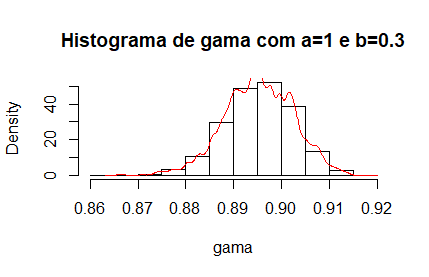
\includegraphics[width=\textwidth]{a1-0b0-3}
 					 \end{subfigure}
 					 \begin{subfigure}[h]{0.6\textwidth}
   						 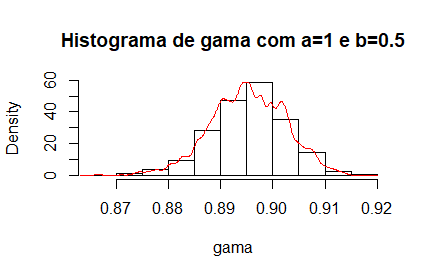
\includegraphics[width=\textwidth]{a1-0b0-5}
 					 \end{subfigure}
 					 \begin{subfigure}[h]{0.6\textwidth}
   						 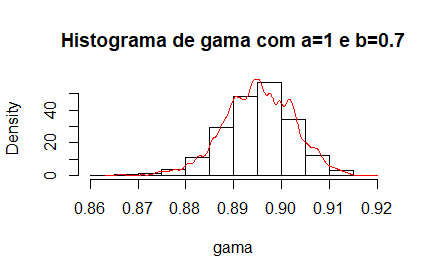
\includegraphics[width=\textwidth]{a1-0b0-7}
 					 \end{subfigure}
 					 \begin{subfigure}[h]{0.6\textwidth}
   						 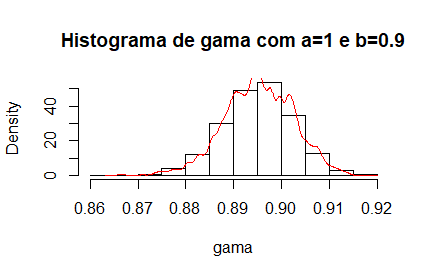
\includegraphics[width=\textwidth]{a1-0b0-9}
 					 \end{subfigure}
 					 \begin{subfigure}[h]{0.6\textwidth}
   						 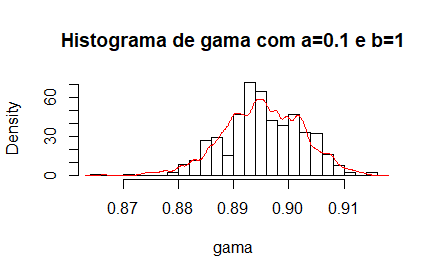
\includegraphics[width=\textwidth]{a0-1b1-0}
 					 \end{subfigure}
 					 \begin{subfigure}[h]{0.6\textwidth}
   						 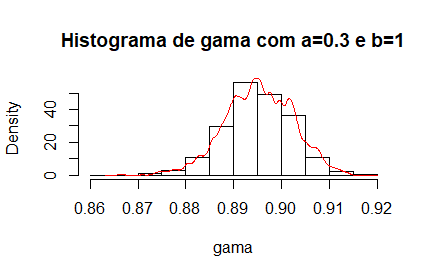
\includegraphics[width=\textwidth]{a0-3b1-0}
 					 \end{subfigure}
				\end{figure}
				\begin{figure}[H]
					 \begin{subfigure}[h]{0.6\textwidth}
   						 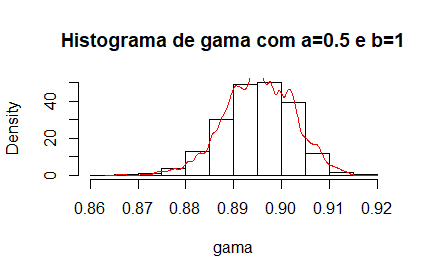
\includegraphics[width=\textwidth]{a0-5b1-0}
 					 \end{subfigure}
 					 \begin{subfigure}[h]{0.6\textwidth}
   						 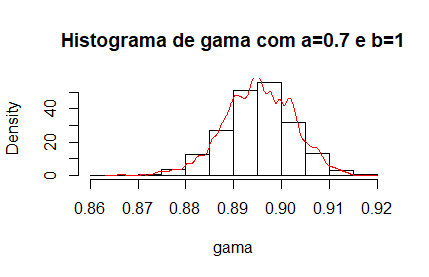
\includegraphics[width=\textwidth]{a0-7b1-0}
 					 \end{subfigure}
 					 \begin{subfigure}[h]{0.6\textwidth}
   						 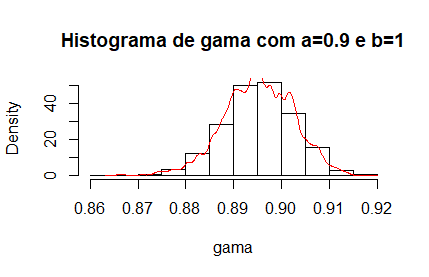
\includegraphics[width=\textwidth]{a0-9b1-0}
 					 \end{subfigure}
					 \begin{subfigure}[sh]{0.6\textwidth}
   						 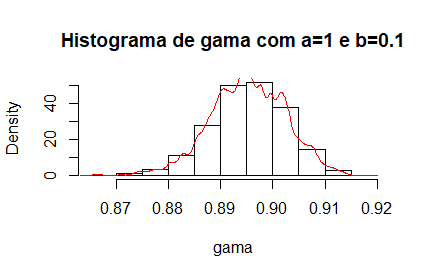
\includegraphics[width=\textwidth]{a1-0b0-1}
 					 \end{subfigure}
				\end{figure}
				\paragraph{}
				
				Ao avaliar os gráficos apresentados anteriormente, podemos verificar que apesar das várias alterações aos valores de \textit{a} e \textit{b}, as distribuições \textit{a posteriori} que aparentam ser distribuições Normal($\mu$, $\sigma^2$), não sofreram grandes alterações em termos de valores gerados. Podemos também observar isso comparando os valores da média e variância gerados nas diferentes distribuições \textit{a posteriori}.

	
\end{document}
